%%%%%%%%%%%%%%%%%项目符号%%%%%%%%%%%%%%%%%%%
\begin{itemize}
\item {\bf 1}...        
\item {\bf 2}...    
\item {\bf 3}...
\item {\bf 4}...
\end{itemize}

%%%%%%%%%%%%%%%%%图片插入%%%%%%%%%%%%%%%%%%%
\begin{figure}[h]   
\centering          
\includegraphics[width=12cm]{"路径"}
\caption{标题} \label{fig1}    
\end{figure}

%%%%%%%%%%%%%%%%%三线表%%%%%%%%%%%%%%%%%%%
\begin{table}[h] 
\centering  
\caption{标题}  
\label{tab1} 
\begin{tabular}{ll} 
\toprule
Symbols  & Descriptions \\    
\midrule 
$S_{P1i}$ & player 1’s momentum integral value in one match\\
$S_{P2i}$ & player 2’s momentum integral value in one match\\
$A_r$   & service score rate                             \\
$F_r$   & service failure rate                           \\
$B_r$   & break success rate                             \\
$B_{fr}$  & break failure rate                             \\
$N_r$   & net scoring rate                               \\
$E_r$   & error ratio                                    \\ 
$T_s$   & the total number of serve in the set           \\
$M$     & momentum                                       \\
\bottomrule
\end{tabular}
\end{table}

%%%%%%%%%%%%%%%%%插图两张图片%%%%%%%%%%%%%%%%%%%
\begin{figure}[H]
    \centering
    \begin{subfigure}{0.45\textwidth}
        \centering
        \includegraphics[width=\textwidth]{图1路径}
        \caption{Player 1's Momentum}
        \label{subfig:player1}
    \end{subfigure}
    \hfill
    \begin{subfigure}{0.45\textwidth}
        \centering
        \includegraphics[width=\textwidth]{图2路径}
        \caption{Player 2's Momentum}
        \label{subfig:player2}
    \end{subfigure}
    \caption{标题}
    \label{Figure 13}
\end{figure}

%%%%%%%%%%%%%%%%%插图公式%%%%%%%%%%%%%%%%%%%
\begin{equation} \label{1}
    M=\sum_{i=1}{6}W_{i}\times\beta _{i}
\end{equation}

%%%%%%%%%%%%%%%%%插入四张图片%%%%%%%%%%%%%%%%%%%
\begin{figure}[htbp]
    \centering
    % 减少顶部间距
    \vspace{-0.15in}
    
    % 第一行两张图片
    \begin{minipage}{1\linewidth}
        \subfloat[]{\label{fig:2.1}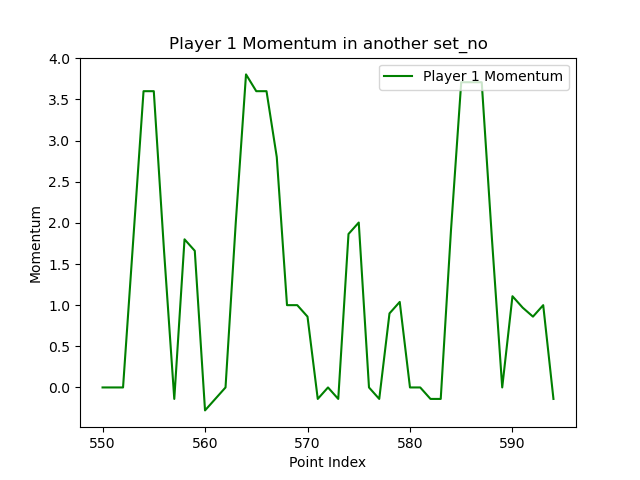
\includegraphics[width=0.45\linewidth]{2.1.png}}
        \hfill % 水平填充
        \subfloat[]{\label{fig:2.2}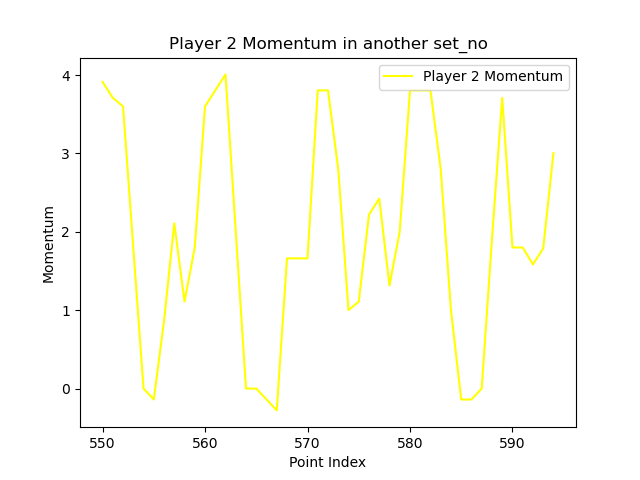
\includegraphics[width=0.45\linewidth]{2.2.png}}
    \end{minipage}
    
    % 减少两行图片之间的间距
    \vskip -0.3cm
    
    % 第二行两张图片
    \begin{minipage}{1\linewidth}
        \subfloat[]{\label{fig:2.3}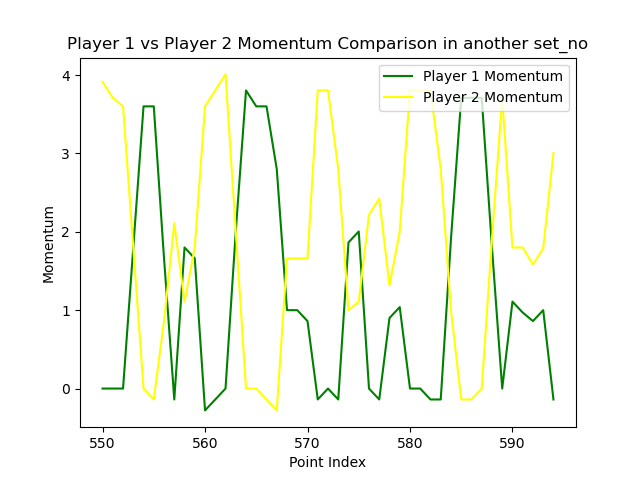
\includegraphics[width=0.45\linewidth]{2.3.png}}
        \hfill % 水平填充
        \subfloat[]{\label{fig:2.4}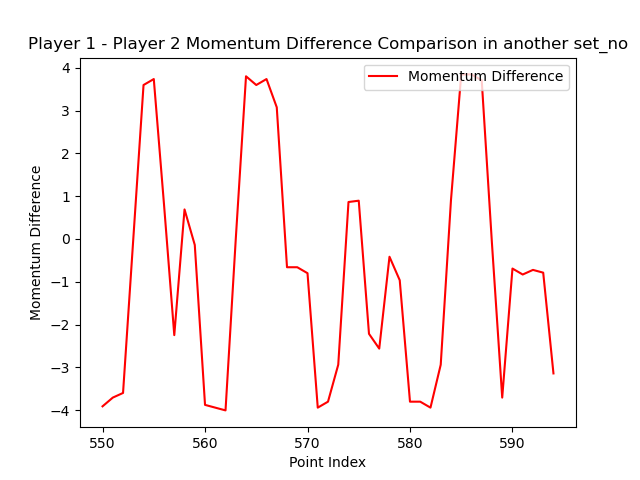
\includegraphics[width=0.45\linewidth]{2.4.png}}
    \end{minipage}
    
    % 减少底部间距
    \vspace{-0.18in}
    
    \caption{Model Application Diagram} \label{fig:8-11}
\end{figure}

